\section Funktionale Anforderungen

Im Fogenden werden wir die Funktionalen Anforderung an unser Programm
erläutern. Diese waren zum Teil durch die Aufgabenstellung gegeben,
ergaben sich aber auch während der Programmierarbeit.
\begin{description}
\item [{Optionale~Verknüpfung~von~Randstücken:}] Wird ein Gitternetz
eines Quaders gezeichnet, so entstehen doppelte Linien, obwohl es
dies Kanten nur einmal gibt. Hier galt es eine Regel zu finden um
Ungenauigkeiten zu vermeiden.
\item [{Unterstützung~der~Anfangszuordnung:}] Bevor mit dem Zeichnen
begonnen wird, sollen die Startpunkte auf den einzelnen Schachteln
ausgewählt werden können.
\item [{Automatisierung~der~Verarbeitung~verschiedener~Schachteln:}] Es
soll durch den Benutzer ausgewählt werden, welche Schachteln er bearbeten
möchte.
\item [{Automatisches~Auffüllen:}] Das ist ein wenig komplizierter, wird
an einer Stelle etwas weggenommen, weil es zum Beispiel durch eine
ander Fläche übermalt wurde, so sollen automatisch die Zwischenräume
aufgefüllt werden.
\end{description}
Frontend - User Interface - Bedienungsanleitung

Im Folgenden wir die Bedienung des Programmes erläuter. Das Projekt kann unter \url{https://dev.spline.de/svn/CommonUnfold/trunk/} runtergeladen werden. Im Ordner \texttt{src} sollte die Datei \texttt{common_unfolding_draw.py} mit dem Befehl \texttt{python common_unfolding_draw.py} gestartet werden. Im Folgenden wird bschreiben, wie man vorgeht um ein Common Unfold zu finden.


\section{Schachteln erzeugen}

Startet man das Programm, so muss man als erstes Schachteln erzeugen,
die Anzahl kann man frei wählen. Diese Schachtel sollten aus dem gefunden
Common Unfold gefaltet werden können. Bei der Erzeugung kann zwischen
\emph{New By Surface} und \emph{New By Dimension} gewählt werden.
\begin{description}
\item [{New~By~Surface:}] Hier gibt man den Oberflächeninhalt an und
alle Schachteln die diesen Oberflächeninhalt haben werden erzeugt,
wenn es mehr als eine gibt.
\item [{New~By~Dimension:}] Hier gibt man die Breite, Höhe und Tiefe
einer Schachtel an, alle weiteren, die in die gleiche Äquvalenzklasse
fallen werden erzeugt.
\end{description}
Man muss mindestens zwei Schachteln auswählen, zusätzlich kann man
die Rotation der Schachteln angeben, sie werden dabei um ihren Urspung
rotiert.


\section{Zeichnenoberfläche}

Wählt man Schachteln aus und Bestätigt mit OK, so gelangt man zum
Zeichenbereich. Als erstes müssen die Startpunkte festgelegt werden,
dies kann man klicken auf die entsprechende Stelle erreichen oder
mit Eingeben der exakten Koordinaten. Die Eingabe muss mit OK bestätigt
werden.

Die Zeichenoberfläche besteht aus drei Bereichen (1,2,3,4).
\begin{description}
\item [{(1)~Zeichenbereich:}] In diesem Bereich wird gezeichnet, hier
entsteht die neue Grundfläche aus der die links abgebildeten Schachteln
gefaltet werden könne.
\end{description}
\begin{figure}
\noindent \begin{centering}
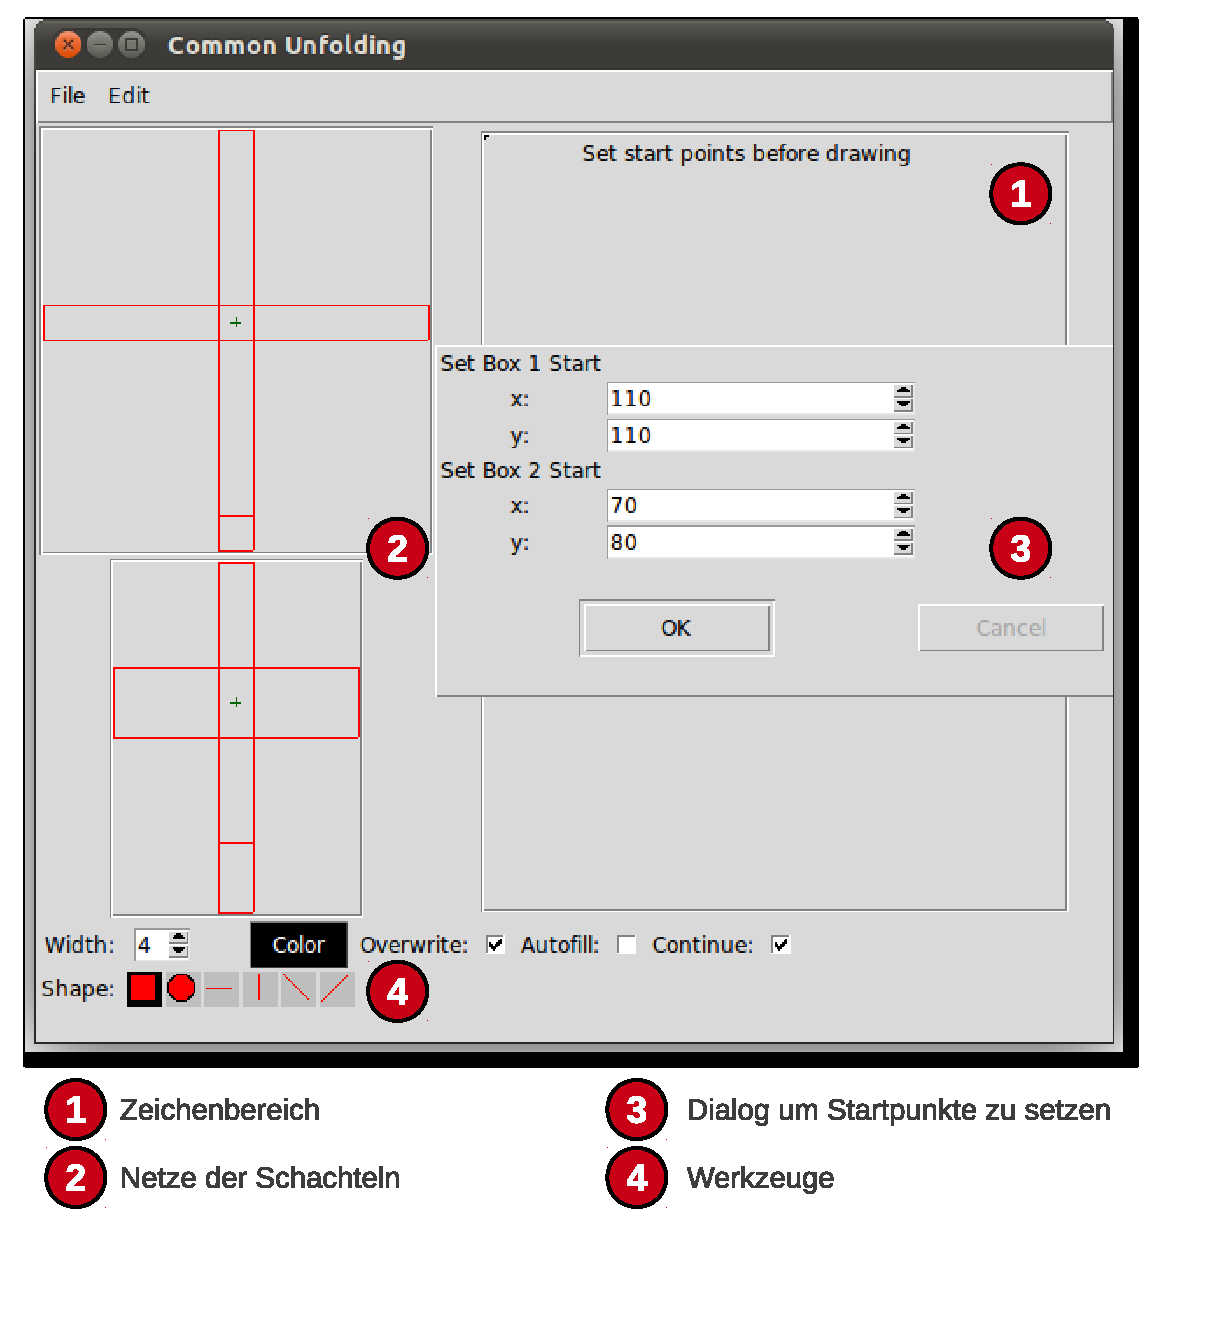
\includegraphics[width=0.5\paperwidth,bb = 0 0 200 100, draft, type=eps]{Zeichenbereich.eps}
\par\end{centering}

\caption{Zeichenoberfläche}


\end{figure}



\section{Datei lade, speichern, exportieren}

Tastenkürzel
\begin{itemize}
\item Beschreibung der Oberfläche, Aufbau des Fensters

\begin{itemize}
\item Wie bedient man das Programm?

\begin{itemize}
\item Wie geht man vor?
\end{itemize}
\item Tastenkürzel und so Sachen
\end{itemize}
\end{itemize}
Technische Umsetzung

allgemeines geplänkel

Wir haben eine Trennung von MVC-Pattern angestrebt. Trennun gvon GUI
und Logik.


\section{Verwendete Technologien}
\begin{itemize}
\item SystemvoraussetzungenCommon unfolding
\item Welches Betreibssystem wird benötigt?

\begin{itemize}
\item Welche Abhängigkeiten sind zu beachten?
\item Wie führe ich das Programm aus?
\end{itemize}
\item 
\item 
\end{itemize}

\section{Frontend - User Interface}

Screenschots, Bereiche erläutern, wie male ich was, vielleicht ein
Beispiel zeigen, was man malen kann


\section{Backend - Softwarearchitektur}

Stichpunkte: 



\selectlanguage{ngerman}%

\subsection{Überblick}

Alle Zeichenvorgänge gehen von einer Benutzereingabe auf der Hauptzeichenfläche
aus, auch beim Zeichnen auf den Schachtel-Zeichenflächen wird ein
entsprechendes Ereignis auf der Hauptfläche ausgelöst, welches in
der draw-Methode des DrawingCanvas-Objektes behandelt wird.

Von den x- und y-Koordinaten dieses Ereignisses ausgehend wird von
jeder Schachtel-Zeichenfläche die Funktion prepare(x, y) aufgerufen.

In den Zeichenflächen werden die Koordinaten berechnet, die, beim
aktuellen Zeichenvorgang, dem Punkt auf der Hauptfläche entsprechen.
Zusätzlich wird angegeben ob dieser Punkt auf der Schachtel-Zeichenfläche
bereits existiert. Falls es auf einer Fläche nicht möglich seien sollte
entsprechende Koordinaten zu berechnen, wird der Zeichenvorgang abgebrochen.

Falls in den berechneten Schachtel-Koordinaten Konflikte aufgetreten
sind, also Punkte auf den Schachtelflächen bereits vorhanden sind,
und das Überschreiben aktiviert ist, werden die bereits vorhandenen
Punkte und ihre entsprechenden Punkte auf den anderen Zeichenflächen
gelöscht. Ein auf der Hauptzeichenfläche bereits vorhandener Punkt
wird ebenso behandelt. Sollte Überschreiben nicht aktiviert sein muss
der Zeichenvorgang bei vorhandenen Konflikten abgebrochen werden.

Nachdem nun mögliche Konflikte behoben sind können alle berechneten
Punkte gezeichnet werden.


\subsection{Berechnen der Schachtel-Koordinaten}

In der Funktion prepare(x, y) der BoxCanvas-Objekte wird von den x-,
y-Koordinaten der Hauptzeichenfläche ausgehend die Koordinaten des
entsprechenden Punktes der Schachtel-Zeichenfläche berechnet.

Ausgehend vom Startpunkt der Schachtelfläche wird eine Verschiebung
der Koordinaten addiert. Falls z. B. der Startpunkt der Hauptfläche
$(100|100)$ ist und der Startpunkt der Schachtelfläche $(200|300)$,
so ergibt sich $(x+100|y+200)$.

Zu jeder Schachtelfläche gehört eine Liste traversed\_edges, in der
die im aktuellen Zeichenvorgang überquerten Kanten gespeichert werden.
Nun wird nacheinander die traverse-Funktion der Kanten für die x-,
y-Koordinaten aufgerufen.

Nun muss festgestellt werden, ob der berechnete Punkt wiederum außerhalb
der Schachtel liegt, ob also eine weitere Kante überquert wurde, oder
ob der Punkt innerhalb der Schachtel liegt. Dazu werden Orientierungstest
mit den Eckpunkten der beiden Rechtecke, die die Schachtelfläche bilden
ausgeführt (Funktion is\_inside(x, y)).

Falls der Punkt außerhalb liegt und im aktuellen Zeichenvorgang bereits
ein Punkt gezeichnet wurde, also ein gültiger Referenzpunkt vorliegt,
wird die zwischen den beiden Punkten liegende Kante festgestellt.
Für diese Kante wird ebenfalls die traverse-Funktion aufgerufen, wodurch
wir wiederum neue Koordinaten erhalten.

Falls kein Referenzpunkt vorhanden ist, kann kein gültiger Punkt berechnet
werden.

Nun haben wir also gültige Koordinaten für einen auf der Schachtel
liegenden Punkt und möglicherweise eine neu überquerte Kante (sollte
der Punkt schließlich gezeichnet werden, wird diese Kante zur Liste
der Überquerten hinzugefügt). Jetzt wird noch geprüft ob der berechnete
Punkt bereits gezeichnet wurde. Diese Information wird zusammen mit
den berechneten Koordinaten zurückgegeben.


\subsection{Automatisches Auffüllen}

Falls auf einer Schachtelfläche ein Punkt gelöscht wird (z. B. aufgrund
von Überschreibung), wird dieser Löschvorgang gespeichert. Nachdem
der aktuelle Punkt gezeichnet wurde, werden die gelöschten Punkt überprüft.
Falls ein Punkt tatsächlich gelöscht wurde, also kein neuer Punkt
an der gleichen Stelle gezeichnet wurde, wird in der Funktion get\_autofill
geprüft, ob auf der entsprechenden Zeichenfläche in der näheren Umgebung
bereits gezeichnet wurde. Die Anzahl der überprüften Pixel ist abhängig
von der eingestellten Zeichenbreite.

Falls ein entsprechender Punkt gefunden wird, wird von diesem aus
{}``aufgefüllt''. Der gelöschte Punkt wird also so gezeichnet, als
wäre er im gleichen Zeichenvorgang entstanden wie der bereits vorhandene
Punkt. 

\selectlanguage{english}%

\subsection{startpunkte (startpoint\_dialog, startpoint\_main)}
\begin{itemize}
\item Startpunkte auf Boxen im startpoint\_dialog mit Mausklick oder in
Spinnbox, box\_canvas.offset wird angepasst Startpunkte auf drawing\_canvas
mit mausklick auf Zeichenfläche in startpoint\_main. startpunkt wird
von allen box\_canvas.offset's subtrahiert
\end{itemize}

\subsection{undo/redo (undoable)}
\begin{itemize}
\item bei draw werden sich alle punkte x,y gespeichrt, wenn vorher gezeichneter
punkt gelöscht wird, werden alle dazugehörigen pixel auf den Boxen
und der Zeichenfläche gespeichert zusätzlich wird der anfangsstatus
gespeichet mit overide, autofill, countinue\_draw und anfangs überquerten
kanten auf den Boxen bei undo werden alle diese punkte mit drawing\_canvas.erase
gelöscht und in der redoliste gespeichert anschließend werden die
durch diese gelöschten pixel vorher überschriebenen pixel wiederhergestellt
\item bei redo wird ein erneutes zeichnen auf der zeichenfläche mit hilfe
von my\_event simuliert
\end{itemize}

\subsection{Speichern/Laden (save\_load)}
\begin{itemize}
\item eine modifzierte Undo-Liste wird abgespeichert als CommonUnfoldFile
{[}{*}.cuf{]}
\end{itemize}

\subsection{CommonUnfoldFile:}
\begin{itemize}
\item int: Anzahl der Boxen Quadtrupel für jede box: (höhe,breite,tiefe,rotation)
tupel für jede box: boxstartpunkt(x,y) tupel: Zeichenflächenstartpunkt
(x,y) int: Anzahl der gezeichneten Linien (Linie endet nach Mausrelease)
für jede linie:\{ int: anzahl der Pixel Boolean: war overwrite aktiv
Boolean: war autofill aktiv Boolean: war continu line aktiv Liste
von Kanten für jede Box als Start boxes.traversed tripel für jeden
Pixel der linie: (x, y, farbe) \}
\item beim laden werden erst die boxen erstellt, dann die startpunkte gesetzt
und dann das zeichnen simuliert
\end{itemize}

\subsection{cursor auf den anderen zeichenflächen anzeigen (cursors)}
\begin{itemize}
\item bind von motion auf der Zeichenfläche und den Boxen auf der zeichenfläche:
kreuz auf der box mit offset erstellen auf einer box: eigen offset
von aktueller position abziehen und auf zeichenfläche kreuz erstellen,
dann für alle anderen boxen mit methode von zeichenfläche kreuze berechnen
\end{itemize}

\subsection{zeichnen auf den Boxen (draw\_from\_box)}
\begin{itemize}
\item rechnet position auf zeichenfläche aus und ruft mit dieser die standart
drawfunktion auf
\end{itemize}

\subsection{zeichendicke und form (choose\_shape, control\_panel, draw\_with,
drawing\_canvas.width\_draw)}
\begin{itemize}
\item für jeden pixel der fläche wird draw aufgerufen
\end{itemize}

\subsection{Generierung der Schachteln und Preview}

...


\subsection{Rotation und Grid}

Projektmanagement und Teamarbeit

Im folgenden Teil des Projektberichtes werde ich auf die Zusammenarbeit
im Team eingehen, Schwierigkeien und Herausforderungen erläutern.


\section{Teammitglieder}

Zu Beginn des Projektes waren wir 4 Teammitglieder: Alexa, Friedrich,
Henry und Michael. Kurz vor Ende des Semesters ist unser Teamkollege
Michael abgesprungen. Wir kannten uns alle nicht, hatten unterschiedliche
Vorerfahrungen, bevorzugten verschiedene Programmiersprachen. Die
Vorraussetzungen erschwerten zu Beginn die Aufgabenverteilung, bzw.
die Einschätzung der Zuverlässigkeit.


\section{Projektmanagemant}

Wir haben uns für das Hosting des Projektes bei Spline{[}Quelle wo
ist das Projekt{]} entschieden. Zur Codeversionierung wird dabei SVN
verwendet Es wird zusätzlich ein Bug-Tracer {[}wo{]} zur Verfügung
gestellt. 

Bei regelmäßigen, wöchentlichen Treffen haben wir über neue Aufgaben
gesprochen, welche wir als Ticket im Trac eingetragen haben. Anschließend
haben wir besprochen, wer welche Aufgabe(n) in der folgenden Woche
übernimmt. Jeder der Fehler entdeckt, sollte diese auch als Ticket
im bugtracker eintragen. Sodass schnell Fehler behoben werden können.


\section{Aufgabenverteilung}

Zusammenfassung


\section{Ergebnisse}


\section{Ausblick}
\begin{itemize}
\item Ausblick (was könnten wir noch machen, welche features brauchen wir
noch, damit das Programm noch besser wird)
\end{itemize}
\bibliographystyle{/home/alexa/Dokumente/din1505/alphadin}
\addcontentsline{toc}{section}{\refname}\bibliography{verweiseCU}